\documentclass[12pt]{article}
\usepackage[a4paper,margin=1in]{geometry}
\usepackage{amsmath,amssymb}
\usepackage{graphicx}
\usepackage{siunitx}
\sisetup{per-mode=symbol}
\usepackage{gvv}

\title{Matrix 2.6.24}
\author{ai25btech11015 -- M Sai Rithik}
\date{}

\begin{document}
\maketitle

\section*{Question (2.6.24)}
Find the area of the parallelogram whose adjacent sides are given by the vectors
$$\Vec{a} = 3\hat{i} + \hat{j} + 4\hat{k} \quad\text{and}\quad \Vec{b} = \hat{i} - \hat{j} + \hat{k}.$$

\section*{Solution}
Consider vectors a and b
\begin{equation}
\Vec{a} = \myvec{3 \\ 1 \\ 4}, \qquad
\Vec{b} = \myvec{1 \\ -1 \\ 1}.
\end{equation}

Magnitude of $\Vec{a}$:
\begin{equation}
\|\Vec{a}\| = \sqrt{3^2 + 1^2 + 4^2} = \sqrt{9 + 1 + 16} = \sqrt{26}.
\end{equation}

Magnitude of $\Vec{b}$:
\begin{equation}
\|\Vec{b}\| = \sqrt{1^2 + (-1)^2 + 1^2} = \sqrt{1 + 1 + 1} = \sqrt{3}.
\end{equation}

Dot product $\Vec{a}\cdot\Vec{b}$ (to get $\cos\theta$):
\begin{equation}
\Vec{a}\cdot\Vec{b} = 
\begin{pmatrix}3 & 1 & 4\end{pmatrix}
\begin{pmatrix}1 \\ -1 \\ 1\end{pmatrix}
= 3\cdot 1 + 1\cdot(-1) + 4\cdot 1 = 3 - 1 + 4 = 6.
\end{equation}

Cosine of the angle:
\begin{equation}
\cos\theta = \dfrac{\Vec{a}\cdot\Vec{b}}{\|\Vec{a}\|\,\|\Vec{b}\|}
= \dfrac{6}{\sqrt{26}\,\sqrt{3}} = \dfrac{6}{\sqrt{78}}.
\end{equation}

Sine of the angle (use $ \sin\theta = \sqrt{1-\cos^2\theta}$):
\begin{equation}
\sin\theta = \sqrt{1 - \left(\dfrac{6}{\sqrt{78}}\right)^{\!2}}
= \sqrt{1 - \dfrac{36}{78}}
= \sqrt{\dfrac{78 - 36}{78}}
= \sqrt{\dfrac{42}{78}}
= \sqrt{\dfrac{7}{13}}.
\end{equation}

Area of parallelogram $= \|\Vec{a}\|\,\|\Vec{b}\|\,\sin\theta$:
\begin{equation}
\text{Area} = \sqrt{26}\,\sqrt{3}\,\sqrt{\dfrac{7}{13}}
= \sqrt{ \dfrac{26\cdot 3 \cdot 7}{13} }
= \sqrt{ \dfrac{26}{13}\cdot 21 }
= \sqrt{2 \cdot 21}
= \sqrt{42}.
\end{equation}

\section*{Final Answer}
\begin{equation}
\boxed{\text{Area} = 6.4807}
\end{equation}

\begin{figure}[h!]
    \centering
    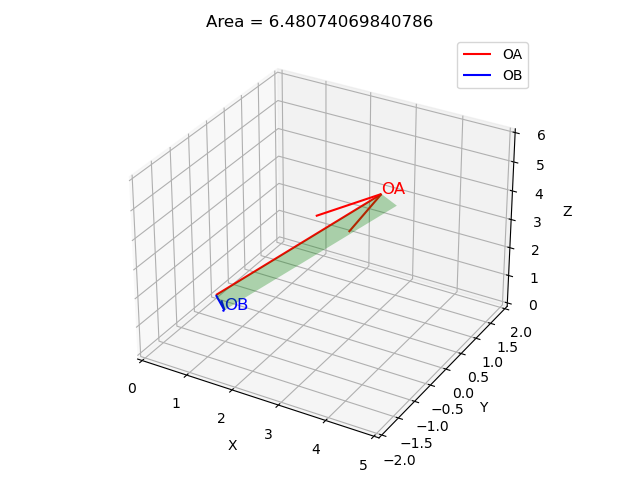
\includegraphics[width=0.6\linewidth]{figs/fig.png}
    \caption{Parallelogram spanned by $\Vec{a}$ and $\Vec{b}$ }
\end{figure}

\end{document}
